\section{Methods and Implementation}
\label{sec:methods}
\fred implements a minimal user interface, Figure \ref{fig:surgery_fred}, to demonstrate registration of a pre-operative image to intra-operative space. At startup a target is placed at a random location within the pre-operative image, shown as a red circle. The standard deviation of the \gls{FLE} is randomly sampled from a uniform distribution 
between 0.5 and 5.0 pixels \footnote{All units are in pixels, as the concepts being explored do not depend on the units used. Figure 
\ref{fig:surgery_fred} shows a brain MRI 458x512 pixels, by design SciKit-SurgeryFRED should work with other images 
of arbitrary dimensions.}. By default the \gls{FLE} is modelled as an isotropic (in 3 dimensions), normally distributed, and independent random variable, though this can be easily changed. 
The variance of the \gls{FLE} is shown to the right of the intra-operative image (as expected value), along with the number of fiducial markers. 

\begin{figure}
	\begin{center}
	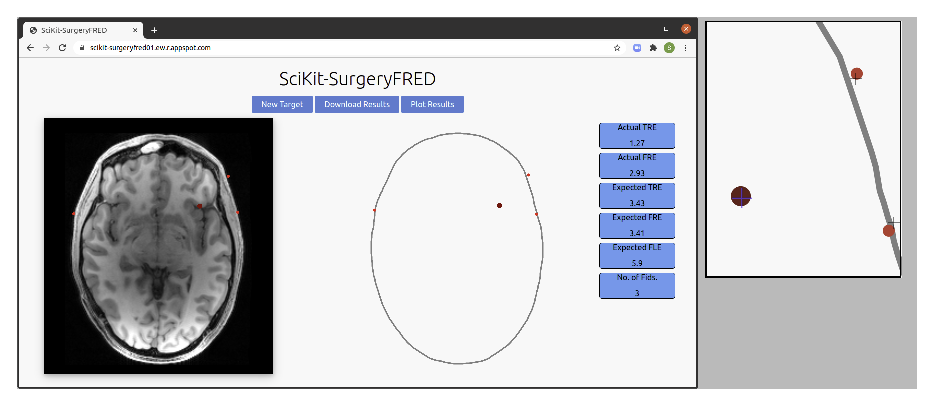
\includegraphics[width=\linewidth]{scikit-surgeryfred_gui.eps}
		\caption{\label{fig:surgery_fred}SciKit-SurgeryFRED graphical user interface after 6 fiducial markers placed. The red circle in the pre-operative image (left) represents a clinical target, which is located in the
		intra-operative space (middle) by fiducial based registration, using the fiducial markers (also red). FLE is added to each marker in the intra-operative image, this is more clearly visible on the zoomed in image at the right. The resulting registration results in a TRE, shown by the misalignment of the red circle and crosshair 
		on the enlarged image at right. TRE and other statistics are shown in boxes to the right of the intra-operative image.}
	\end{center}
\end{figure}

Clicking either image adds a fiducial marker to both images. By default the marker is added to the pre-operative image 
with no \gls{FLE}. \gls{FLE} is added to the marker location in the intra-operative image, visualised as the misalignment
between the red circle centre and the cross-hair. Once sufficient markers are placed ($>2$) the two sets of markers are registered using least squares fitting as described by Arun et al.\cite{Arun1987}. The expected values (variance) of the \gls{FRE} and \gls{TRE} are calculated 
using equations described by Fitzpatrick et al.\cite{Fitzpatrick1998}. The student can use this interface together with an 
online tutorial 
to explore the relationships between the various statistics and error measures. The
user can keep adding as many fiducial markers as they like for a given target. 
Pressing the ``New Target'' button will place a new target at a random position 
within the pre-operative image and randomly sample a new standard deviation for the
\gls{FLE}.

It is straightforward to explore how both \gls{TRE} and \gls{FRE} change in response to 
both the number and geometry of the fiducial markers as is well established in the literature\cite{1295074, Fitzpatrick1998}. 
It is
also simple and instructive to create degenerate marker geometries, for example 
a linear arrangement can produce low \gls{FRE} but extreme values of \gls{TRE}.

During use the registration results are 
stored in the browser. At any time the user can press the ``Plot Results'' button to quickly create a set of 
plots showing the relationship between the actual \gls{TRE} and the various statistics. 
An example plot is shown in Figure \ref{fig:correlation}. 
The student is usually able to see first hand that, as expected, \gls{FRE} is uncorrelated with \gls{TRE}. 

\begin{figure}
	\begin{center}
	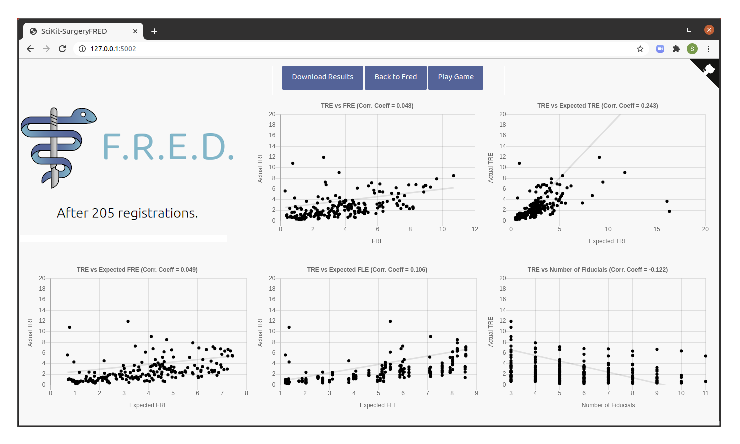
\includegraphics[width=0.9\linewidth]{images/default.eps}
		\caption{\label{fig:correlation}Plots of TRE against various error measures, generated by 
		205 user registrations.}
	\end{center}
\end{figure}

\fred does not implement tests of statistical significance to avoid excessive software dependencies, so it is often 
useful for the students to download the registration results and perform some statistical analysis. This is facilitated by the 
``Download Results'' button which allows the user to get the results as a file in comma separated variable format. 
For example the results in Figure \ref{fig:correlation} may prompt some students to ask if there is in fact a correlation 
between \gls{FRE} and \gls{TRE}, as there is an apparent though slight increase in \gls{TRE} with \gls{FRE}. This can quickly 
be dispelled by asking the student to download the results and perform a test of significance on the data. 

\subsection{Game Based Usability Study}
\label{sec:game_method}
Once the students have an understanding of what statistics can be used to estimate \gls{TRE}, we wanted to test 
how knowledge of a particular statistic affects optimal treatment planning. We designed a serious game to 
do this. During this game the students are asked to perform a registration with a maximum of 
6 fiducial markers, then set a treatment margin and ablate the target. The goal is 
to treat 100\% of the target with minimal ablation of surrounding tissue.
A score of 1000 was awarded for complete ablation and 0 
for anything less. From this starting score 10 times the percentage volume of any
surrounding tissues ablated is subtracted. 
Successful treatments (100\% ablation) should therefore score between 0 and 1000, with a larger margin giving a lower score.
The optimum (minimum successful) treatment
margin is the actual \gls{TRE} for a given registration. 
Any treatment that fails to treat 100\% of the target will receive a negative score. 

Each student participated in the game, performing 20 simulated ablations. For the first four ablations they were told the 
actual \gls{TRE} for training and to supply baseline data. After that they performed 16 more ablations and were shown one of four randomly selected statistics on which to base their decision,
the expected values of the \gls{TRE}/\gls{FRE}, the actual \gls{FRE}, the expected value of the \gls{FLE}. These statistics
were chosen as these are either known or can be estimated for a clinical procedure. Each statistic was shown 4 times, though
the order was randomised for each participant. The scores for each ablation were recorded,  yielding 20 data points for 
each participant.

\subsection{Software Implementation}
\fred is part of the \sksurgery\cite{PMID:32436132} family of libraries. In common with \sksurgery the majority of \fred is implemented in Python. Python was chosen as it combines sufficient features for clinical
applications such as the SmartLiver system\cite{PMID:32780240}, whilst remaining easy enough for students to learn and contribute to. 
In contrast, although platforms built using {C\raisebox{0.5ex}{\tiny\textbf{++}}} provide power and 
flexibility, the choice of language creates a barrier to learning the key concepts of image guided surgery \cite{surgineering}. A key design goal of 
\sksurgery is to keep individual libraries compact and orthogonal\cite{pragmaticprog}, simplifying dependency structures. Based on 
analysis using cloc\footnote{\href{https://github.com/AlDanial/cloc}{https://github.com/AlDanial/cloc} [v1.82]} \fred consists of 802 lines of Python 
code. The user interface is implemented in HTML5 and JavaScript, enabling multiple simple deployment 
options. Again, using cloc, there are 561 lines of HTML5 and JavaScript. These numbers are similar to the other \sksurgery libraries which typically have around 2000 lines of code \cite{PMID:32436132}. In comparison, this paper consists of around 420 lines of Latex code.

Figure \ref{fig:dependencies} shows the direct dependencies of \fredns. The key functional dependency is
\core\cite{matt_clarkson_2020_3965731}. \core implements matched point based registration \cite{Arun1987} together 
with the calculation of expected \gls{FLE} and \gls{TRE}
(equations 10 and 31 from Fitzpatrick et al.\cite{Fitzpatrick1998}). 
{NumPy} \cite{2020NumPy-Array} is used for array handling.
Flask\footnote{\href{https://palletsprojects.com/p/flask/}{https://palletsprojects.com/p/flask/}  [v1.1.2]} provides the web application framework 
to enable the browser based user interface to communicate with the Python based back end. The user
interface communicates with the back end with a series of {POST} requests. All state information is stored in the 
browser front end, allowing the back end to remain stateless, simplifying deployment. 
Including the Google Cloud FireStore API\footnote{\href{https://pypi.org/project/google-cloud-firestore/}{https://pypi.org/project/google-cloud-firestore/} [v2.0.1]} 
enables the optional storage of results in a remotely hosted database. Plotting functionality is implemented
using Chart.js\footnote{\href{https://www.chartjs.org/}{https://www.chartjs.org/} [v2.9.4]}

\begin{figure}
	\begin{center}
	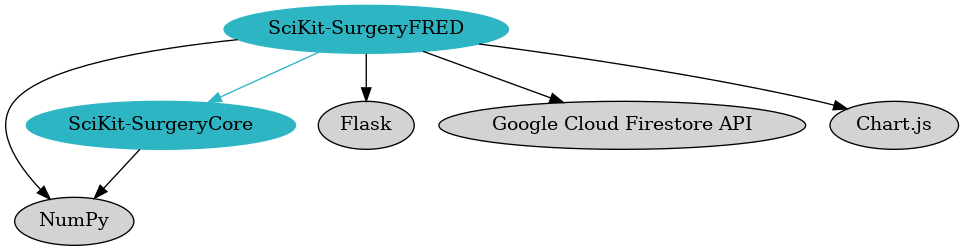
\includegraphics[width=0.7\linewidth]{dependency_graph.eps}
		\caption{\label{fig:dependencies}Software dependencies of SciKit-SurgeryFRED. The registration algorithms and statistical measures of {TRE} are imported from SciKit-SurgeryCore and are shared with clinical applications built on SciKit-Surgery. The user interface is a Flask based web application, using Chart.js for plotting functionality.}
	\end{center}
\end{figure}

In common with the rest of \sksurgery \fred utilises extensive testing and software process \cite{1398621} to 
ensure the application is robust, reusable, and sustainable\cite{VENTERS2018174}. Change control and issue tracking is managed
on GitHub\footnote{\href{https://github.com/UCL/scikit-surgeryfred}{https://github.com/UCL/scikit-surgeryfred}} and continuous integration is managed using
GitHub Actions.

\subsection{Availability and Usage}
For those who want to quickly try \fredns, we currently maintain a running instance hosted at \href{https://scikit-surgeryfred.ew.r.appspot.com/}{https://scikit-surgeryfred.ew.r.appspot.com/}. This should be accessible from most modern web browsers.

If you want to run a locally hosted instance, or modify the code for your needs, you can download the source code. \fred is entirely open source software and is tested on Linux, MacOS, and Windows. The latest version can be obtained from Github. Alternatively, archived releases can be retrieved via Zenodo\cite{stephen_thompson_2020_4314971}.

\begin{lstlisting}[language=bash]
	git clone https://github.com/UCL/scikit-surgeryfred
\end{lstlisting}

Once installed the dependencies can be installed on a local virtual machine using tox. The application can then be run with as follows. This should output a web address that you can open in a browser to run the software. 

\begin{lstlisting}[language=bash]
	cd scikit-surgeryfred
	tox
	source .tox/py37/bin/activate
	python main.py
\end{lstlisting}

\subsection{Extension to Anisotropic Errors}
\label{sec:anis_method}
In many cases {FLE} cannot be properly modelled as an isotropic, independent, random variable. In the case of optical tracking systems for example \cite{10.1117/12.536128} the errors normal to the camera plane are approximately 3 times those parallel to the camera plane. It is straightforward to implement such an anisotropic \gls{FLE} in SciKit-SurgeryFRED and test the effect on registration outcomes.
The following code snippet is taken from  main.py. Line 63 defines the ratio of \gls{FLE} in three directions. By default they are all equal.

\begin{lstlisting}[language=python, firstnumber = 54]
@app.route('/getfle', methods=['POST'])
def getfle():
    """
    Returns values for fiducial localisation errors
    Values are randomly selected from a uniform
    distribution from 0.5 to 5.0 pixels
    """
    fle_sd = np.random.uniform(low=0.5, high=5.0)
    #change fle_ratio if you want anisotropic fle
    fle_ratio = np.array([1.0, 1.0, 1.0], dtype=np.float64)
    anis_scale = math.sqrt(3.0 / (np.linalg.norm(fle_ratio) ** 2))
    fixed_fle = fle_ratio * fle_sd * anis_scale

    moving_fle = np.array([0., 0., 0.], dtype=np.float64)
    fixed_fle_eavs = expected_absolute_value(fixed_fle)
    moving_fle_eavs = expected_absolute_value(moving_fle)

    returnjson = jsonify({
            'fixed_fle_sd': fixed_fle.tolist(),
            'moving_fle_sd': moving_fle.tolist(),
            'fixed_fle_eav': fixed_fle_eavs.tolist(),
            'moving_fle_eav': moving_fle_eavs.tolist()
            })
    return returnjson
\end{lstlisting}

Changing line 63 to;
\begin{lstlisting}[language=python, firstnumber=63]
    fle_ratio = np.array([3.0, 1.0, 1.0], dtype=np.float64)
\end{lstlisting}
sets the error in the x direction to 3 times that in the y and z directions.  

\subsection{Addition of Systematic Errors}
\label{sec:sys_method}
A second significant source of error that is usually overlooked is the presence of systematic errors. For example when using a tracked pointer for fiducial localisation, 
any pointer calibration error will be be added to all fiducial markers.
Similarly some optical tracking systems can introduce a systematic error on 
the tracking markers \cite{6294449}. \fred allows systematic error to 
be added to each fiducial. The fiducial localisation error is set within 
the JavaScript function init{\textunderscore}fles()
(defined in static/main.js) each time a new target is set. 
\begin{lstlisting}[language=java, firstnumber = 429]
/**
 * Sets the global fiducial localisation error (FLE)
 */
function init_fles() {
  fetch("/getfle", {
      method: "POST",
    })
    .then(resp => {
      if (resp.ok)
        resp.json().then(data => {

        let preOpFLEStdDev = data.moving_fle_sd;
        let intraOpFLEStdDev = data.fixed_fle_sd;
        let preOpFLEEAV = data.moving_fle_eav;
        let intraOpFLEEAV = data.fixed_fle_eav;

        let preOpSysError = [0.0, 0.0, 0.0];
        let intraOpSysError = [0.0, 0.0, 0.0];

        FLE = { preOpFLEStdDev, intraOpFLEStdDev,
                preOpFLEEAV, intraOpFLEEAV,
                preOpSysError, intraOpSysError };

      });
    })
    .catch(err => {
      console.log("An error occured setting fles", err.message);
    });
}
\end{lstlisting}
By default there is no systematic error, (lines 445 and 446). We can 
add a systematic interoperative error at line 446 as; 

\begin{lstlisting}[language=java, firstnumber = 446]
        intraOpSysError = [1.0 * (Math.random()-0.5), 
                           1.0 * (Math.random()-0.5), 
                           1.0 * (Math.random()-0.5)];
\end{lstlisting}

In this case the error is an isotropic uniform random variable, in the range
-0.5 to 0.5. This error will be applied to all fiducial markers for a 
given registration. 


